\section{Fast Cycle: Outliner Detection Model}\label{sec:fastCycle}
In this section, we introduce a classification model that takes into account both $F_c$ and $F_s$. 

\subsection{Related Features}\label{relatedFeatures}


\subsubsection{Scientific Measurements $F_s$:}
Blood pressure, SPO2, EKG, and body temperature are standard scientific features that can be easily measured by sensors. 
Usually, they can be accurately measured. Also, there are also standard value boundaries for determining abnormal values. 

\subsubsection{Chinese Medicine Measurements $F_c$:}
Tongue, fatigue, weak breadth, pulse, sweaty are 5 traditional Chinese medicine measurements that can be felt or sensed by 
people themselves or determined by Chinese medicine physicians. However, the values felt or sensed by people themselves 
may sometimes be subjective. 

\subsubsection{Personal Information $F_p$:}
Sex, age, and race are useful personal information that can be use to distinguish a person's health reasonable health condition 
since people with different sex, age, and race usually have different normal values for $F_s$ and $F_c$. 

\subsection{Methodology}

% \subsection{Feature Correlation}
% Our first step is to find out the correlation between features and the label (type of crime). 
% In case features are highly correlated to the label, we will try to build the model by directly adopting 
% some classification models (e.g. Decision Tree). 

\subsubsection{Outliner Detection for $F_c$}\label{sec:outliner}
Firstly, all people are separated into group based on their $F_p$. 
Secondly, all data points that are within the same group are put into a multi-dimensional space based on $F_c$. 
The center point $c$ of these data point is the mean of all data points. 
We regard all data points that are $\tau$ from the center point as outliners and the other $p\%$ as normal data points. 
$\tau$ is a parameter that can be determined based on related medical literatures. 

\begin{equation}
  M_c=\begin{cases}
    1, & \text{if $dist(F_c,c) \geq \tau$}.\\
    0, & \text{otherwise}.
  \end{cases}
\end{equation}
,where $1$ indicate abnormal and $0$ indicates normal.

In Figure~\ref{fig:outliner}, people with $F_p=\{M,20-30,Asian\}$ are put into 
the same group and $p$ is set to $95\%$. Hence, all red dots are regarded as outliners. 

\begin{figure}[ht]
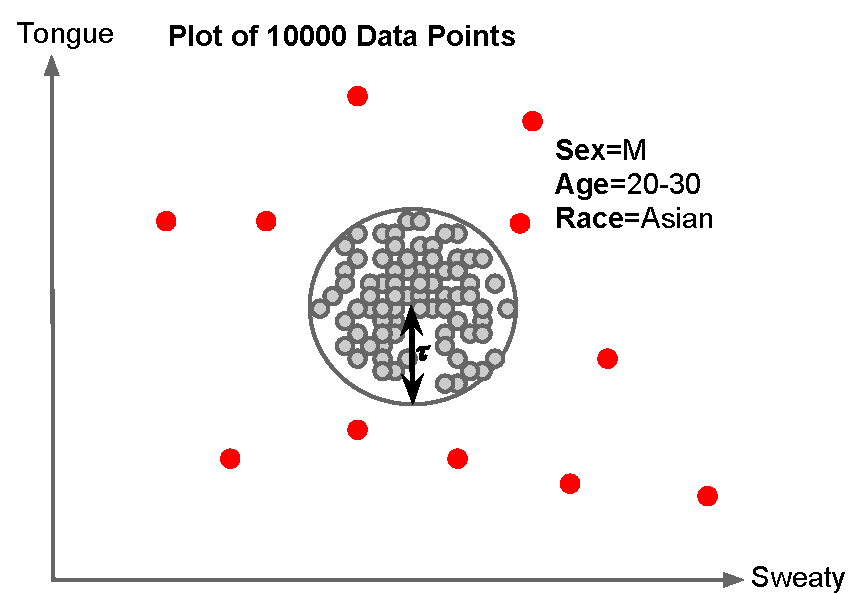
\includegraphics[width=0.9\columnwidth]{experiment/outlinerDetection-crop}
\caption{Outliner Detection}
\label{fig:outliner}
\end{figure}

\subsubsection{Model using $F_c$ and $F_s$}
$M$ is a model for fast cycle. 
We regard every parameter in $F_s$ as a $M_i^s$. $M_i^s$ is $1$ 
if the value is an abnormal value based on $F_p$ of that person; 
otherwise, $M_i^s$ is $0$. 

\begin{equation}
  M_i^s=\begin{cases}
    1, & \text{if $F_s$ is abnormal, given $F_p$}.\\
    0, & \text{otherwise}.
  \end{cases}
\end{equation}

$$M=max(M_c,M_1^s,M_2^s,M_3^s,M_4^s)$$

Parameters of $M_c$ are determined based on feeling and experience of people. 
Therefore, it is possible that error may occur. 
$M_i^s$ and abnormal boundaries of them are scientific measurements. 
Therefore, even $M_c$ is $0$, if any $M_i^c$ is $1$, we should still regard $M$ as $1$ (abnormal). 